\chapter{Implementation}
\label{chap:imp}
\lhead{\emph{Project Implementation}}
% This chapter should comprise 15 pages and enumerate your experience when doing what you wanted to do the way you wanted to do it.

\section{Difficulties Encountered}
% Enumerate the different difficulties you have found when developing your solution approach. Create three categories of difficulties:
    % \item \textbf{Easy}: You managed to solve the problem with little difficulty.
    % \item \textbf{Medium}: It was not easy to solve, but you managed to develop a workaround or solution and still achieve the functionality you originally had in mind.
    % \item \textbf{Hard}: The difficulty was so complicated that you didn’t managed to solve it. As a result, some functional requirement / non-functional requirement or use case from your solution approach was not achieved.

    Developing NoteReader involved navigating a range of technical and architectural challenges. These difficulties can be grouped into three categories: Easy, Medium, and Hard, depending on the complexity of the problem and the extent to which a successful resolution was achieved.

    \subsection{Hard: Framework Immaturity and Document Rendering}
        
    
        One of the most significant challenges was the relative immaturity of Kotlin Multiplatform. The first long-term support stable version was only released in November of 2023. While the framework offers exciting features and remains a solid choice for the requirements of NoteReader, it does introduce several new technical challenges. 

        
        \subsubsection{Nature of Difficulty}
            \begin{enumerate}
                \item
                As the framework is so new, Kotlin Multi-platform has a smaller community, with a smaller based of established resources when compared to more mature alternatives like Flutter or React. 
                \item
                I found that official documentation and forum discussions were insufficient to resolve issues, necessitating trial-and-error experimentation.
                \item
                The ecosystem surrounding Kotlin Multiplatform, particularly the third-party libraries available on platforms like Klibs.io (Jetbrains' official repository for community libraries and plug-ins), is still developing. Many libraries were either incomplete, poorly documented, or lacked support for key features required by the project. This was especially problematic for modules related to document parsing and rendering.
          \end{enumerate}  
    
            
        \subsubsection{Effect on the original project design:}
            \begin{enumerate}
                \item The original intended architecture was to implement fully independent rendering module for each document type. Each module would implement a standard interface allowing each rendering path to be slotted in to the same pipeline.
                \item
                True-to-intent rendering of documents is a core principle of the project, so it was important to make sure the document looks like it should. Images should appear where the author placed them, font sizes and other formatting should also match. 
                \item
                I had originally intended to use drop in solutions where possible to achieve this, but I found that many of the community built options available on Klibs.io we not sufficient. Most community options were either experimental or lacked critical functionality, such as accurate page rendering or support for embedded multimedia.

            \end{enumerate}
    
                
        \subsubsection{Approach to solve difficulty}
            \begin{enumerate}
                \item I experimented with several different approaches to solve this difficulty. Starting by adapting Java or Android-specific libraries into the project.
                
                \item One solution I attempted was parsing the documents directly and rendering them as html and css in a web view. I abandoned this approach due to scalability concerns, as it would require bespoke implementations for each document type. With the focus being on wide ranging document format support, this would massively increase the development cost of each format. 
        
                \item One community library which worked very well was the  \hyperlink{https://github.com/zt64/compose-pdf/tree/main}{compose-pdf library created by developer zt64 and offered under an MIT license}. This library provided an excellent starting point as a PDF renderer. 
                
                \item Ultimately I settled on the approach of converting all supported document type to a temporary PDF file at run-time. The original file remains unchanged and is preserved for archival purposes. The generated PDF is then passed to the compose-pdf renderer for display.
        
                \item Converting various document types to pdf is a very common workflow, so there was a greater level of support available online to help in developing this solution. That said, there remained very few options available for Kotlin Multiplatform Specifically. 
        
                \item As the programming language Kotlin is built on Java, it is cross compatible. I was able to use several Apache libraries, including POI to parse Microsoft documents such as PowerPoint and word, along with  PDFBox to generate the PDFs. 
        
                \item Certain file types were not as easily converted with existing embeddable libraries however. I chose to integrate two free and open source binary programs into the workflow. LibreOffice, is an office suite which includes open source alternatives to popular products like Microsoft Office, Excel, and Power Point. Calibre is an open source e-reader. 
                
                Both LibreOffice and Calibre offer a portable version, each giving access to a wealth of command line tools in pre-compiled binaries, which can be integrated into the Kotlin Multiplatform application. 
                
                Calibre was used to convert e-books formats (such as epub), While LibreOffice was used to convert legacy Microsoft formats. 
    
            \end{enumerate}
    
    
            With the above solution, all of the document types planned for the prototype were implemented. Pdf, Docx, Doc, Pptx, Epub and Html. 

            This architecture allowed for faithful rendering of diverse document types across all target platforms while maintaining extensibility for future format support.
    

    % % For each difficulty, classify it into easy, medium or hard. Then, provide the following info:
    % \begin{enumerate}
    %     \item Description of the difficulty: Brief description of the problem you found.
    %     \item How did it affect the original project design?: Indicate how this difficulty affected:
    %     \begin{enumerate}
    %         \item the architecture of your solution
    %         \item if it represented a risk to your project
    %         \item if it affected your methodology to develop your project
    %         \item if it changed your implementation schedule
    %         \item if it changed the evaluation plan
    %     \item What did you do to manage the difficulty arisen?: Brief description of your decision to overcome the difficulty.
    %     \end{enumerate}
    % \end{enumerate}


\section{Actual Solution Approach}
\label{sec:actual_solution}

This section presents a reflective comparison between the original solution design, as proposed in Chapter 4, and the final implementation delivered at the end of the development phase. From January to May, the project evolved through iterative development, guided by the original architecture, use cases, and methodology. 

However, as with most software projects, practical challenges, such as framework limitations, time constraints, and unexpected technical hurdles, necessitated adjustments to the initial plan. What follows is a structured, component-by-component analysis that documents these changes, explains the underlying causes, and evaluates the decisions made to ensure a functioning and maintainable end product. Each subsection outlines the intended design, contrasts it with what was ultimately delivered, and provides a rationale for any divergences observed.

\subsection{Architecture Comparison}
\subsubsection{Original Design}
The original architecture proposed for NoteReader was structured around a modular, cross-platform framework using Kotlin Multiplatform. 

The core logic was intended to be platform-agnostic, with separate implementations for UI and rendering components for each target platform (Windows, macOS, Linux, and Android). The application followed a Model-View-Controller (MVC) paradigm to promote separation of concerns and ease of maintenance. 

Several methods were proposed as potential options for rendering documents, often revolving around embedded web views for formats such as PDF and EPUB, and markdown notes were to be stored in plain-text files with metadata managed via a local index or catalogue. Synchronization with GitHub or GitLab was planned through integrated version control utilities.

\subsubsection{Final Implementation}
The final implementation closely adheres to the architectural plan outlined in the original design, particularly in its modular structure and use of Kotlin Multiplatform. 

The core logic and data handling remain abstracted from the UI layer, and Compose Multiplatform has been successfully used to build out the desktop front end. 

The application includes a dual-pane layout with PDF rendering in one pane and markdown-based note editing in the other. Notes are saved in lightweight plain-text files, and the application state is persisted using a JSON-based structure.

However, only the desktop version has been implemented thus far. Platform-specific renderers for mobile and Linux systems were not developed in this phase due to time constraints and the complexity of supporting diverse file formats across environments. Synchronization functionality via Git was also not implemented. 


\subsubsection{Key Changes and Rationale}

The most notable deviation from the original architecture was the decision to focus exclusively on the desktop platform. This decision was driven primarily by limited development time. The project is however designed with expansion in mind, structured in such a way to make it simple to add additional platforms without changing the core program. 

Additionally, the reliance on web views for document rendering proved less mature than expected requiring fallback to slower but more reliable conversion pipelines in some cases.

Another key architectural adjustment was the temporary omission of the Git synchronization module. Although the file structure and catalogue system were built to support version-controlled syncing, integrating Git APIs introduced significant complexity that could not be addressed within the available timeframe.

In summary, while the core architecture remained faithful to the original design, practical limitations led to a reduction in scope and simplification of some components. The system remains extensible and modular, ensuring that postponed features, such as cross-platform UI layers and Git integration, can be added in future development cycles without requiring fundamental refactoring.


\subsection{Risk Assessment Revisited}
\subsubsection{Original Risk Matrix}

\begin{table}[h]
\centering
\scriptsize
\caption{Initial risk matrix}
\begin{tabular}{|p{2cm}|p{2cm}|p{2cm}| p{2cm} |p{2cm}| p{2cm}|}
\hline \bf Frequency/ Consequence & \bf 1-Rare & \bf 2-Remote & \bf 3-Occasional & \bf 4-Probable & \bf 5-Frequent\\ [10pt]

\hline \bf 4-Fatal & \cellcolor{yellow!50} & \cellcolor{red!50} & \cellcolor{red!50} & \cellcolor{red!50} &\cellcolor{red!50} \\ [10pt]

\hline \bf 3-Critical &\cellcolor{green!50} & \cellcolor{yellow!50} & \cellcolor{yellow!50} & \cellcolor{red!50} &\cellcolor{red!50} \\ [10pt]

\hline \bf 2-Major & \cellcolor{green!50} & \cellcolor{green!50} & \cellcolor{yellow!50} &\cellcolor{yellow!50} &\cellcolor{red!50} \\ [10pt]

\hline \bf 1-Minor & \cellcolor{green!50} & \cellcolor{green!50} & \cellcolor{green!50} &\cellcolor{yellow!50} &\cellcolor{yellow!50} \\ [10pt]
\hline
\end{tabular} \\
\label{tab:ProjRisks}
\end{table}

\begin{table}[h]
\centering
\caption{Risk Table for Identified Risks}
\begin{tabular}{|l|c|c|}
\hline
\textbf{Risk}                           & \textbf{Frequency} & \textbf{Consequence} \\
\hline
\rowcolor{yellow!50} Scope Creep        & Occasional        & Major                 \\
\hline
\rowcolor{red!50} File Corruption       & Remote            & Fatal                 \\
\hline
\rowcolor{yellow!50} Merge Conflicts    & Frequent          & Minor               \\
\hline
\rowcolor{green!50} Large File Sizes   & Rare              & Major                 \\
\hline
\end{tabular}
\label{tab:ProjRisks}
\end{table}

\subsubsection{New Risks Identified}

\begin{table}[h]
\centering
\caption{Risk Table for Newly Identified Risks}

\begin{tabular}{|l|c|c|}
\hline
\textbf{Risk}                           & \textbf{Frequency} & \textbf{Consequence} \\
\hline
\rowcolor{yellow!50} Framework Learning Curve        & Occasional        & Major                 \\
\hline
\rowcolor{yellow!50} Third-Party Library Limitations        & Occasional        & Critical                 \\
\hline
\rowcolor{red!50} Time Constraints and Parallel Commitments        & Frequent        & Major                 \\

\hline
\end{tabular}
\label{tab:ProjRisks}
\end{table}

\begin{itemize}
    \item \textbf{Framework Learning Curve:}  
    Although Kotlin Multiplatform was selected for its cross-platform promise, working with an emerging framework like Compose Multiplatform introduced a steeper learning curve than anticipated. Documentation gaps, platform inconsistencies, and immature tooling led to delays, particularly in rendering components and file handling workflows.

    \item \textbf{Third-Party Library Limitations:}  
    Availability of plugins and libraries compatible with kotlin multiplatform was limited due to the immaturity of the platform. Early dependencies, such as those used in the web view approach were found to have constraints not initially evident during the design phase. Issues with third party libraries and the added development cost of bespoke implementations resulted in a need to redesign parts of the file processing logic.

    \item \textbf{Time Constraints and Parallel Academic Commitments:}  
    As this project was conducted alongside academic coursework, available development hours were sometimes inconsistent, especially around assignment and exam periods. This impacted velocity and required periodic rescoping of deliverables to match remaining capacity.
\end{itemize}

\subsubsection{Mitigation Measures Adopted}
\begin{itemize}
    \item \textbf{Prioritization of Core Features:}  
    To address the effects of scope creep, development efforts were re-centered around the primary user flow: importing, reading, and annotating documents. Secondary features such as Git integration, tagging, and advanced search were deprioritized and marked for future iterations. This ensured that the minimum viable product (MVP) remained deliverable within the timeline.
    
    \item \textbf{Fallback Conversion Methods:}  
    To mitigate issues with EPUB and DOCX rendering, fallback strategies such as conversion to PDF or plain-text extraction were introduced. While not as elegant as native rendering, this ensured compatibility and allowed users to continue engaging with their content.


    \item \textbf{Interface Abstraction for Platform Readiness:}  
    Although cross-platform support was not fully achieved during this phase, the codebase was structured using interface-driven design. Platform-specific implementations are abstracted, allowing new targets (e.g., Android or macOS) to be added later without refactoring the core application logic.
    
    \item \textbf{Use of Git for Incremental Backup and Rollback:}  
    Even though user-facing Git integration was not finalized, Git was used throughout development to manage version control of the codebase. This provided resilience against code loss, enabled rollback of unstable changes, and served as a lightweight progress tracking mechanism.

    \item \textbf{User Interface Simplification:}  
    To improve usability despite time and platform constraints, the UI was deliberately simplified. Large buttons, color-coded panes, and minimal navigation steps reduced the learning curve and made the application usable with minimal training or documentation.


\end{itemize}

\subsection{Methodology Execution}
\subsubsection{Planned Development Methodology}
The project was originally planned using the Agile Scrum methodology, with an emphasis on iterative development and incremental feature delivery. The development timeline was broken down into six two-week sprints, each with a specific focus:

\begin{itemize}
    \item Sprint 1: Document rendering (PDF) and linked note-taking editor.
    \item Sprint 2: Catalogue implementation and document/note retrieval.
    \item Sprint 3: Expanded file format support (EPUB, DOCX, PPTX).
    \item Sprint 4: Synchronization system design (Git integration).
    \item Sprint 5: UI/UX refinement and accessibility testing.
    \item Sprint 6: Prototype integration, testing, and documentation.
\end{itemize}

\subsubsection{Adaptations Made During Implementation}
In general Sprints took longer to complete than initially planned. 

From an early stage it was clear that the scope of the project needed to be reigned in to focus on only core features. Sprint 2 was changed to Focus on File System and Program State, while Sprint 3 was changed to Expanding file format support, which was the area where most difficulties were encountered. As a result this sprint took much longer than originally hoped. 

Git integration and the Catalogue system were pushed to future development cycles. 

Overall after all adjustments there were 5 Sprints across the semester: 

\begin{itemize}
    \item \textbf{Sprint 1:} Document rendering (PDF) and linked note-taking editor.
    \item \textbf{Sprint 2:} Focus on File System and Program State
    \item \textbf{Sprint 3:} Expanded file format support (EPUB, DOCX, DOC, PPTX, HTML).
    \item \textbf{Sprint 4:} UI/UX refinement.
    \item \textbf{Sprint 5:} Prototype integration and documentation.
\end{itemize}

\subsection{Implementation Timeline}
\subsubsection{Original Sprint Schedule}
Originally planned as 6 two week sprints. 
\subsubsection{Actual Timeline}
\begin{itemize}
    \item \textbf{Sprint 1:} Ending Feb 24th
    \item \textbf{Sprint 2:} Ending Mar 4th
    \item \textbf{Sprint 3:} Ending Apr 8th
    \item \textbf{Sprint 4:} Ending May 5th
    \item \textbf{Sprint 5:} Ending May 20th (on submission of source code)
\end{itemize}

\subsubsection{Deviation Analysis and Justification}
Difficulties were encountered in rendering documents other than PDF, due to immaturity of the platform and lack of available libraries and plug-ins. 

From an early point in development, it was decided to focus on wide ranging File support. Implementation approach needed to change to render these file formats in a manner which respected the authors intent. Exploring and experimenting with available options such as web view and pdf conversion extended the duration of sprints. 

\subsection{Prototyping Outcomes}
\subsubsection{Initial Prototypes}
Several wire frame prototypes were produced in advance of beginning development.  (See appendix:\ref{Wireframes})

An interactive prototype was produced in WPF using C\#, to act as a visual aid (see figure: \ref{fig:NoteReaderMock})

A visual prototype of a mobile interface was produced in JustInMind (see figure \ref{fig:NoteReaderMock2}

\subsubsection{Final Product Interface and Features}
\begin{itemize}
    \item Two Pane layout, featuring Document Reader and Note Editor, with zoom buttons and buttons to navigate between pages (fig:\ref{fig:reader})
    \item Note editor can be swapped to Markdown rendering Layout (fig: \ref{fig:mdView}
    \item Home Screen, Import Documents, Open the folder where files are contained, open imported documents (fig: \ref{fig:home})
    \item Dark Mode, shows potential for theming to user's preference (fig: \ref{fig:dark}
    \item Center Column in Reader View provides buttons which allow you to enter a focus mode for either the Reader or Note Taker,  making that pane take up the full width of the window. Also contains a button which allows you to swap the two panes.
\end{itemize}

\begin{figure}
    \centering
    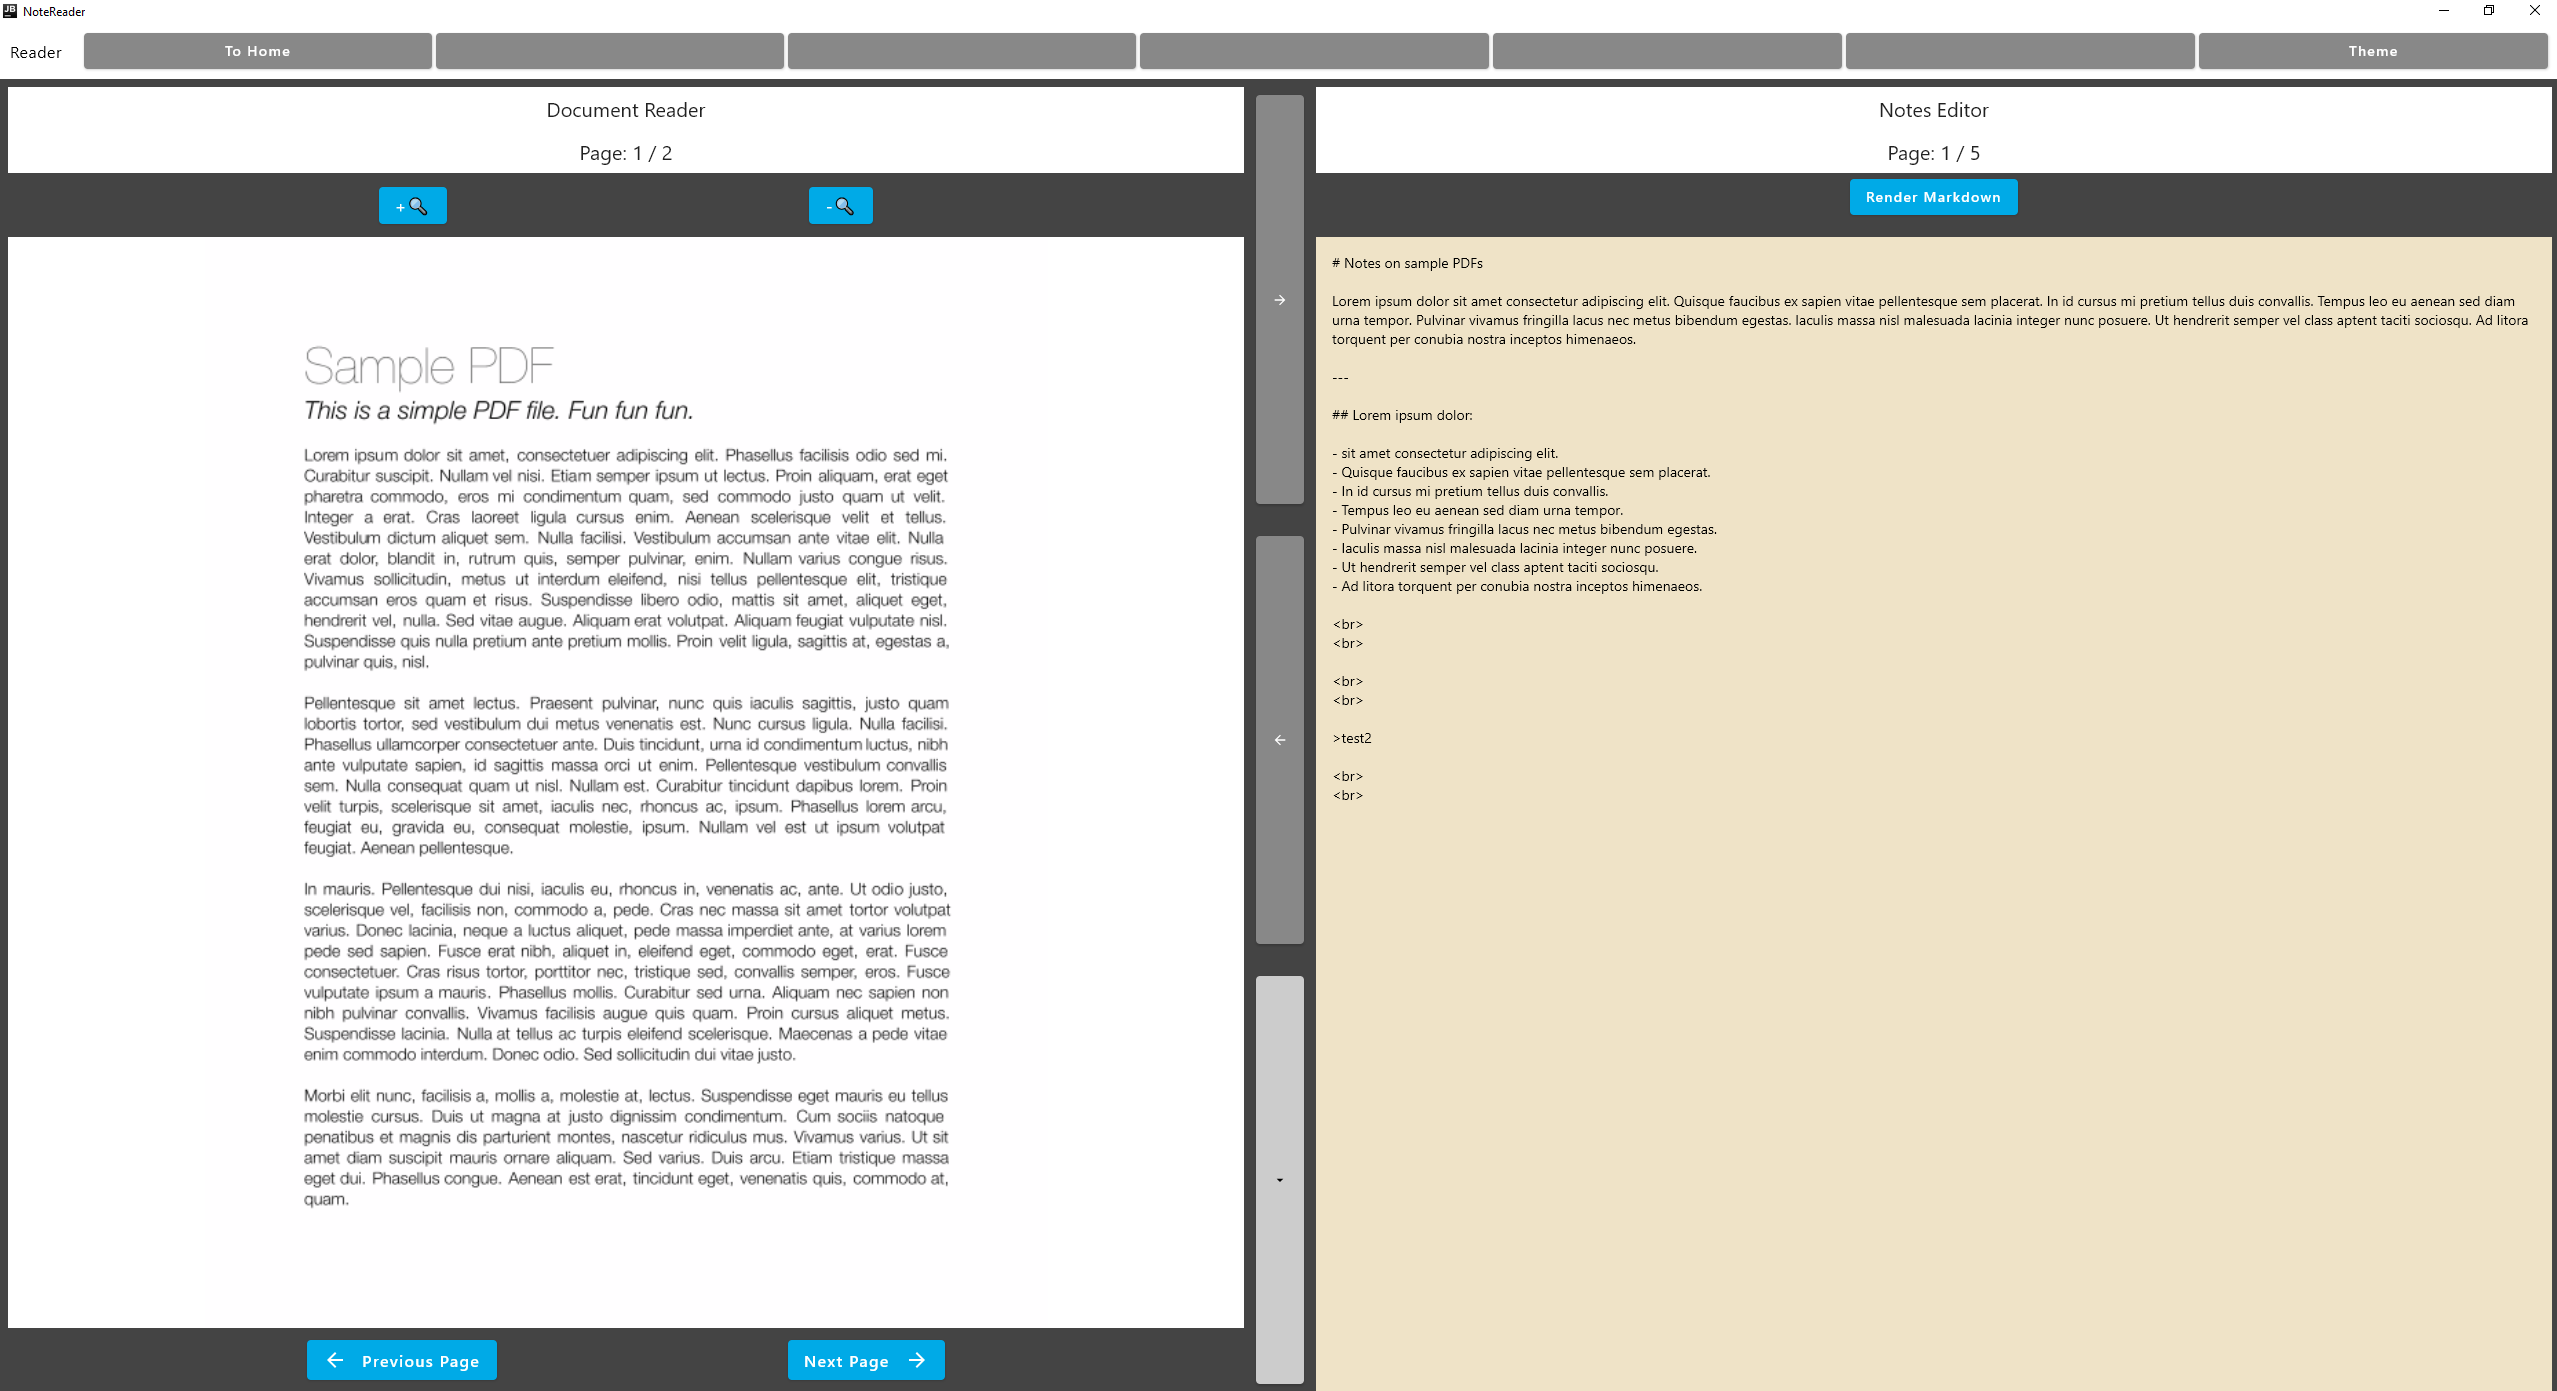
\includegraphics[width=1\linewidth]{image.png}
    \caption{Reader Page}
    \label{fig:reader}
\end{figure}


\begin{figure}
    \centering
    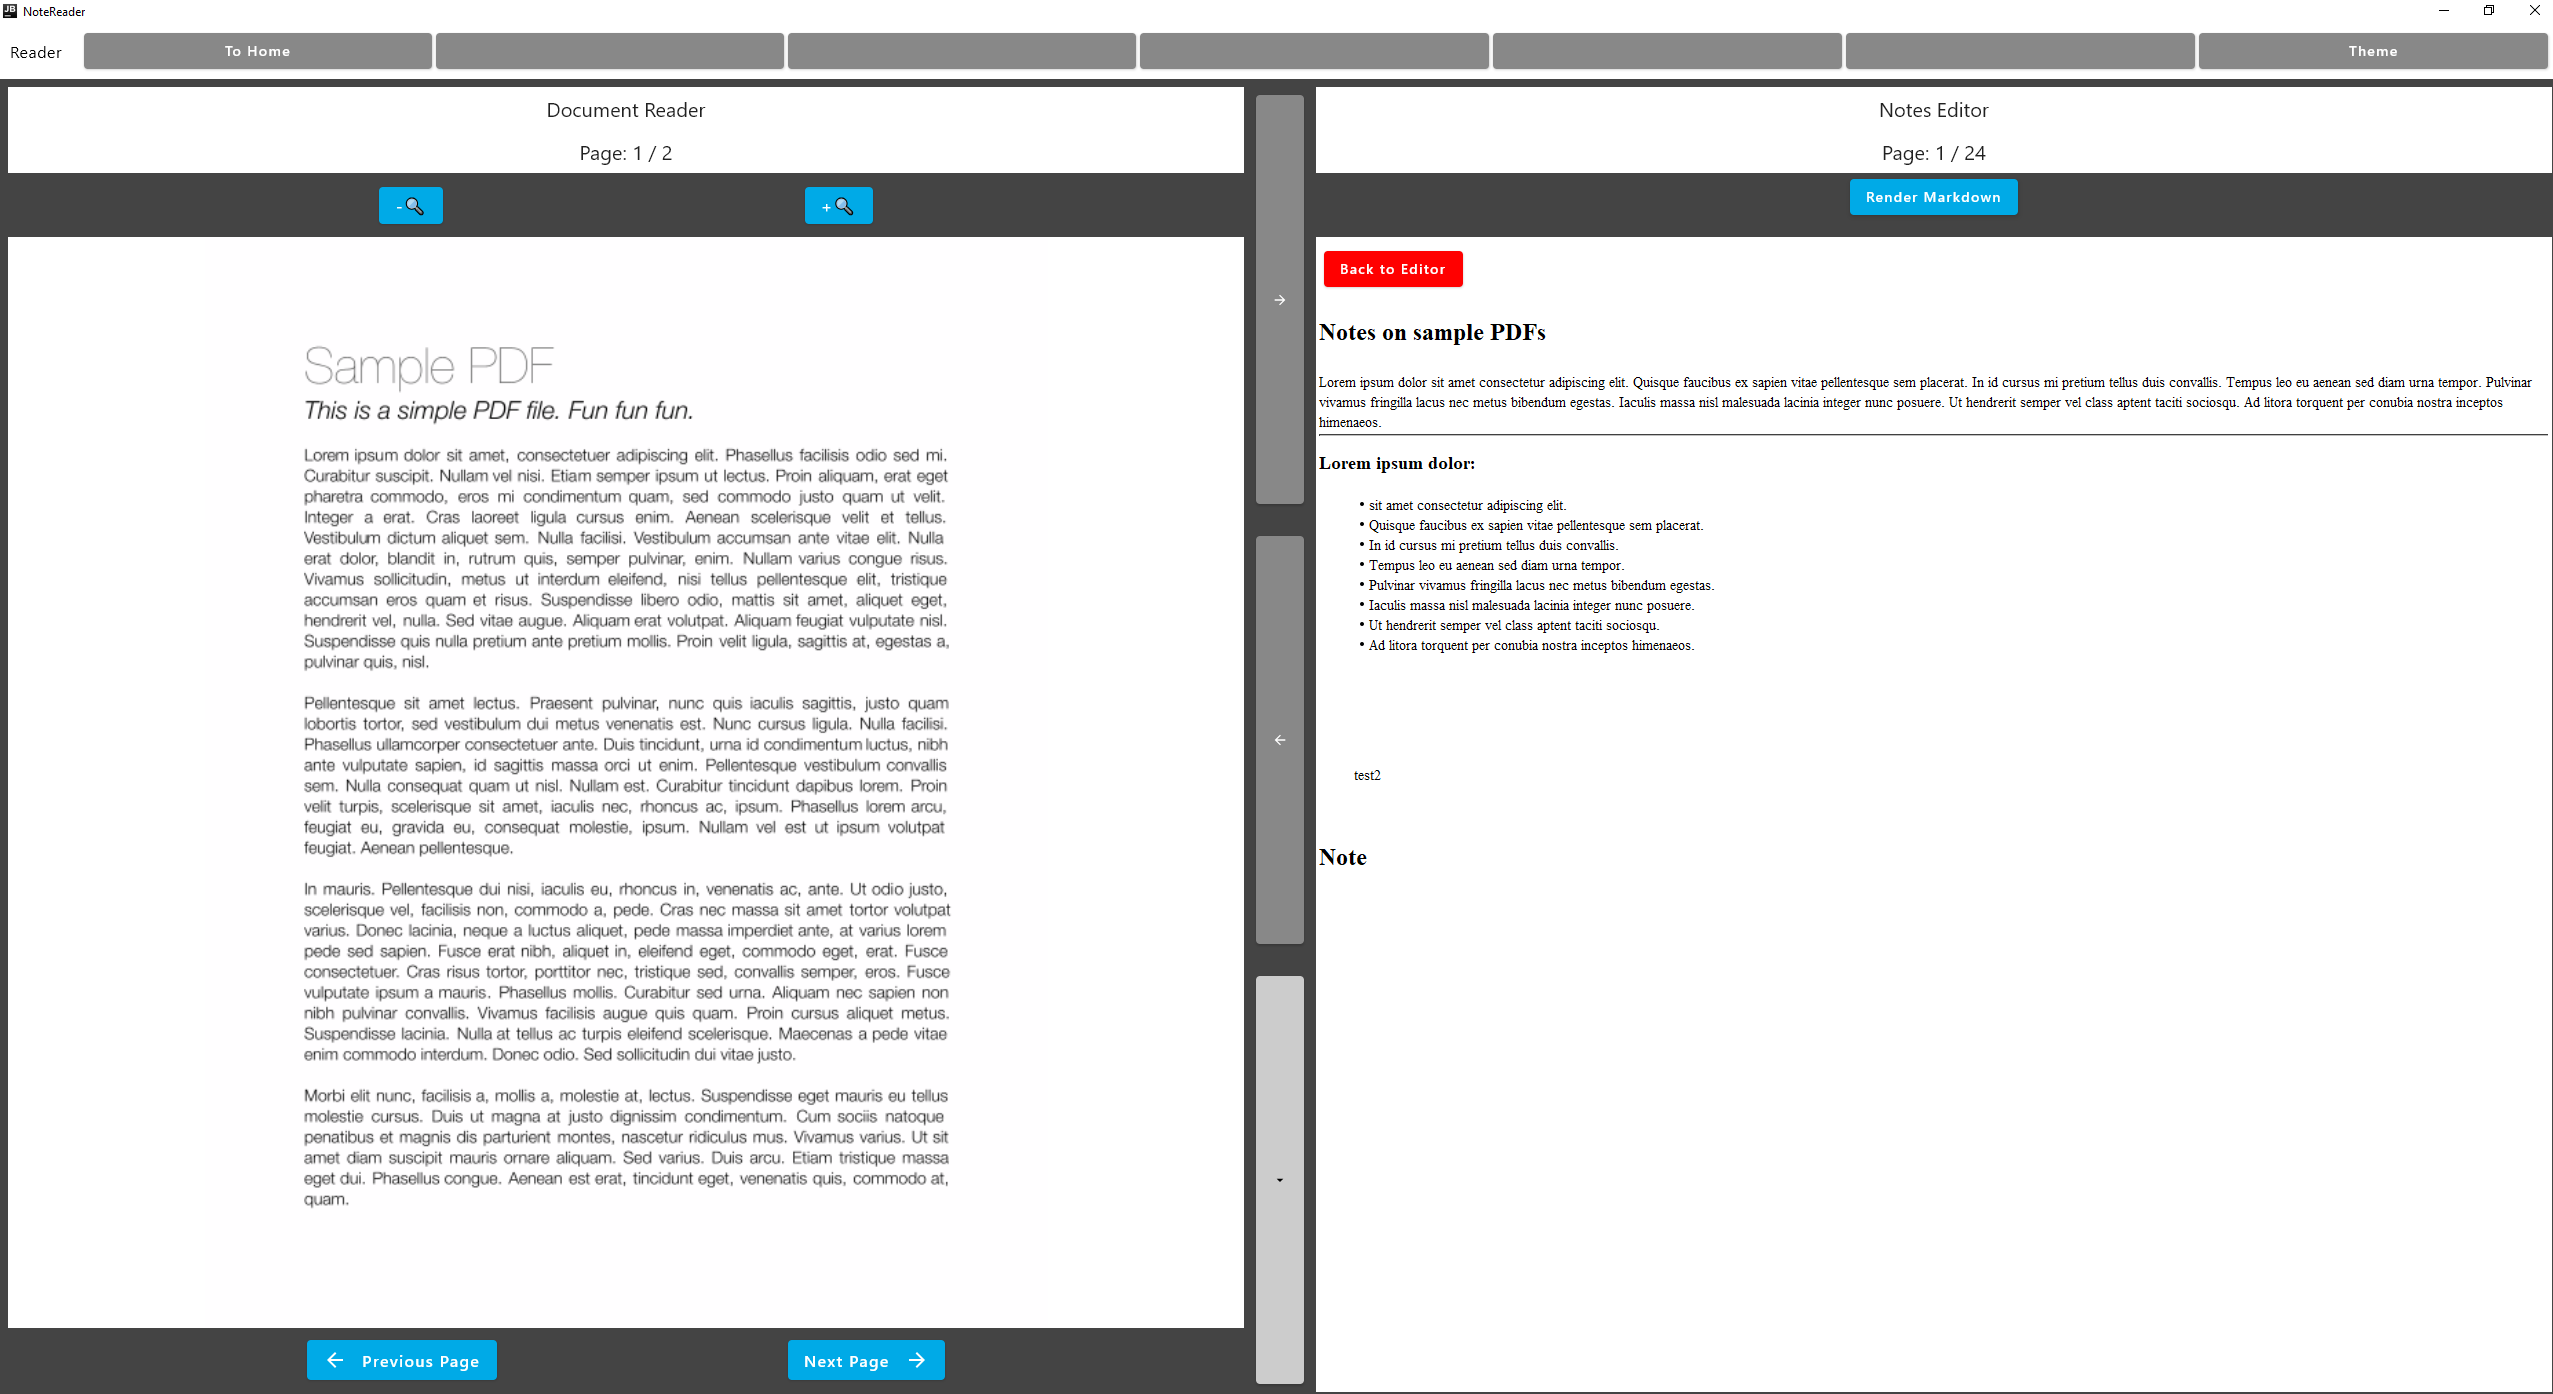
\includegraphics[width=1\linewidth]{Figures/image2.png}
    \caption{Markdown View}
    \label{fig:mdView}
\end{figure}

\begin{figure}
    \centering
    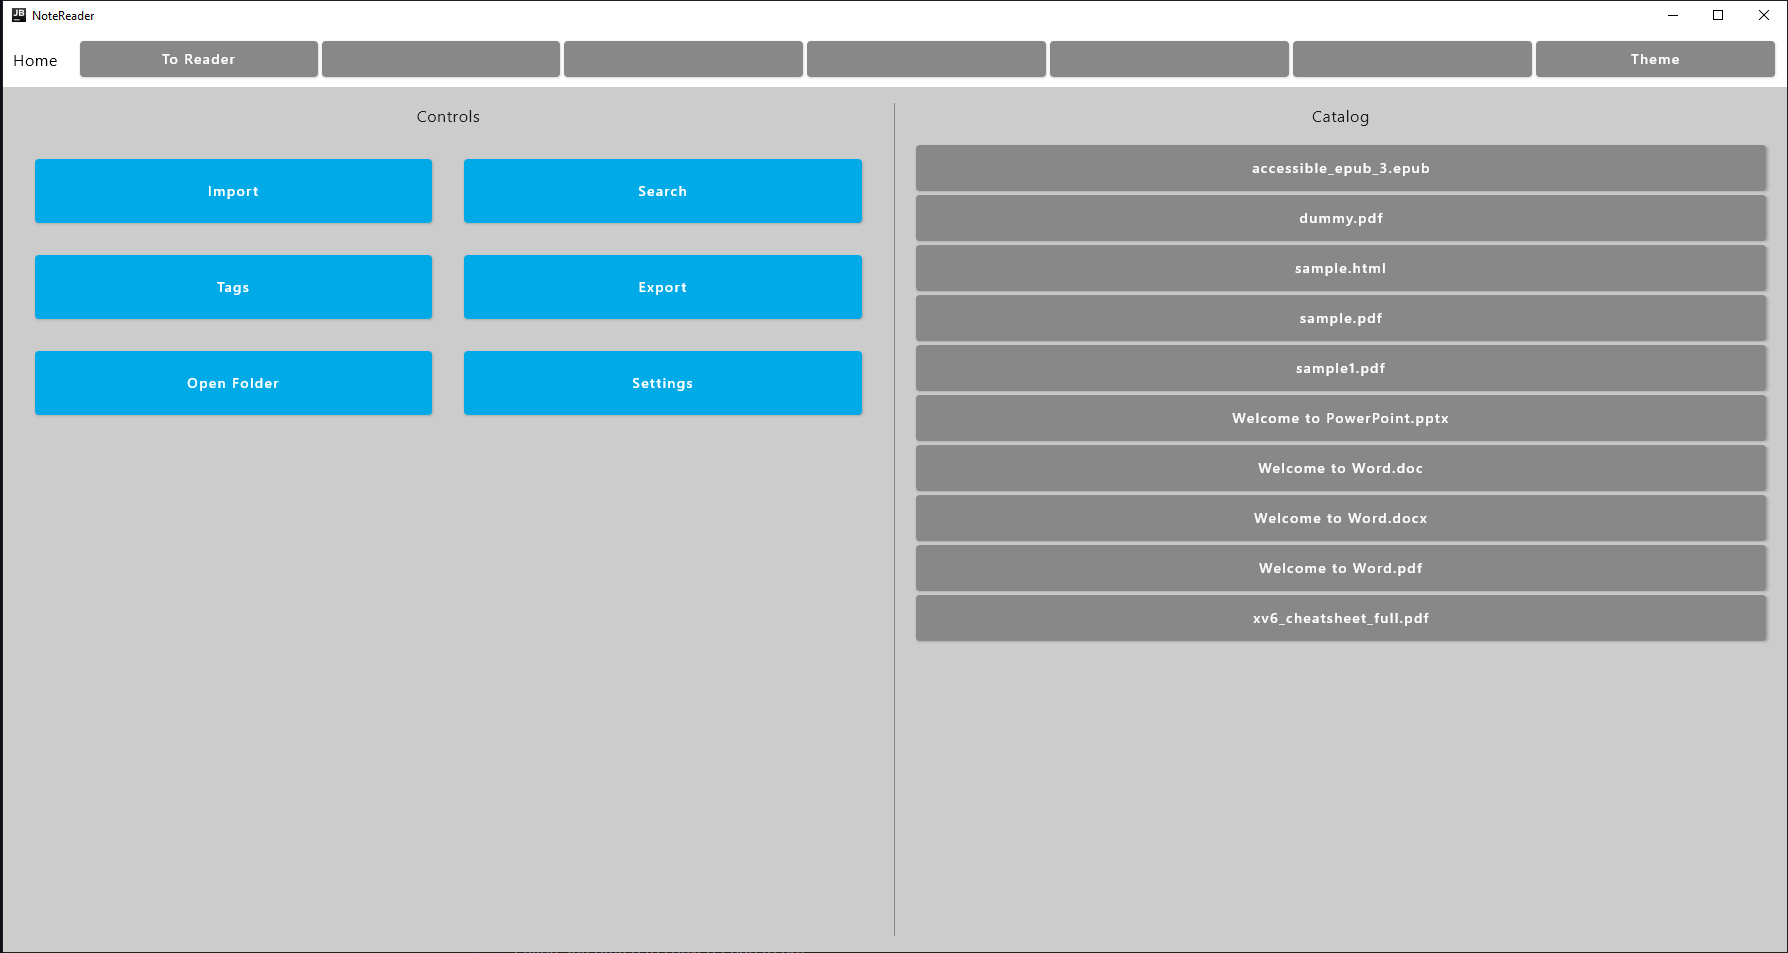
\includegraphics[width=1\linewidth]{Figures/image3.png}
    \caption{Home Screen}
    \label{fig:home}
\end{figure}

\begin{figure}
    \centering
    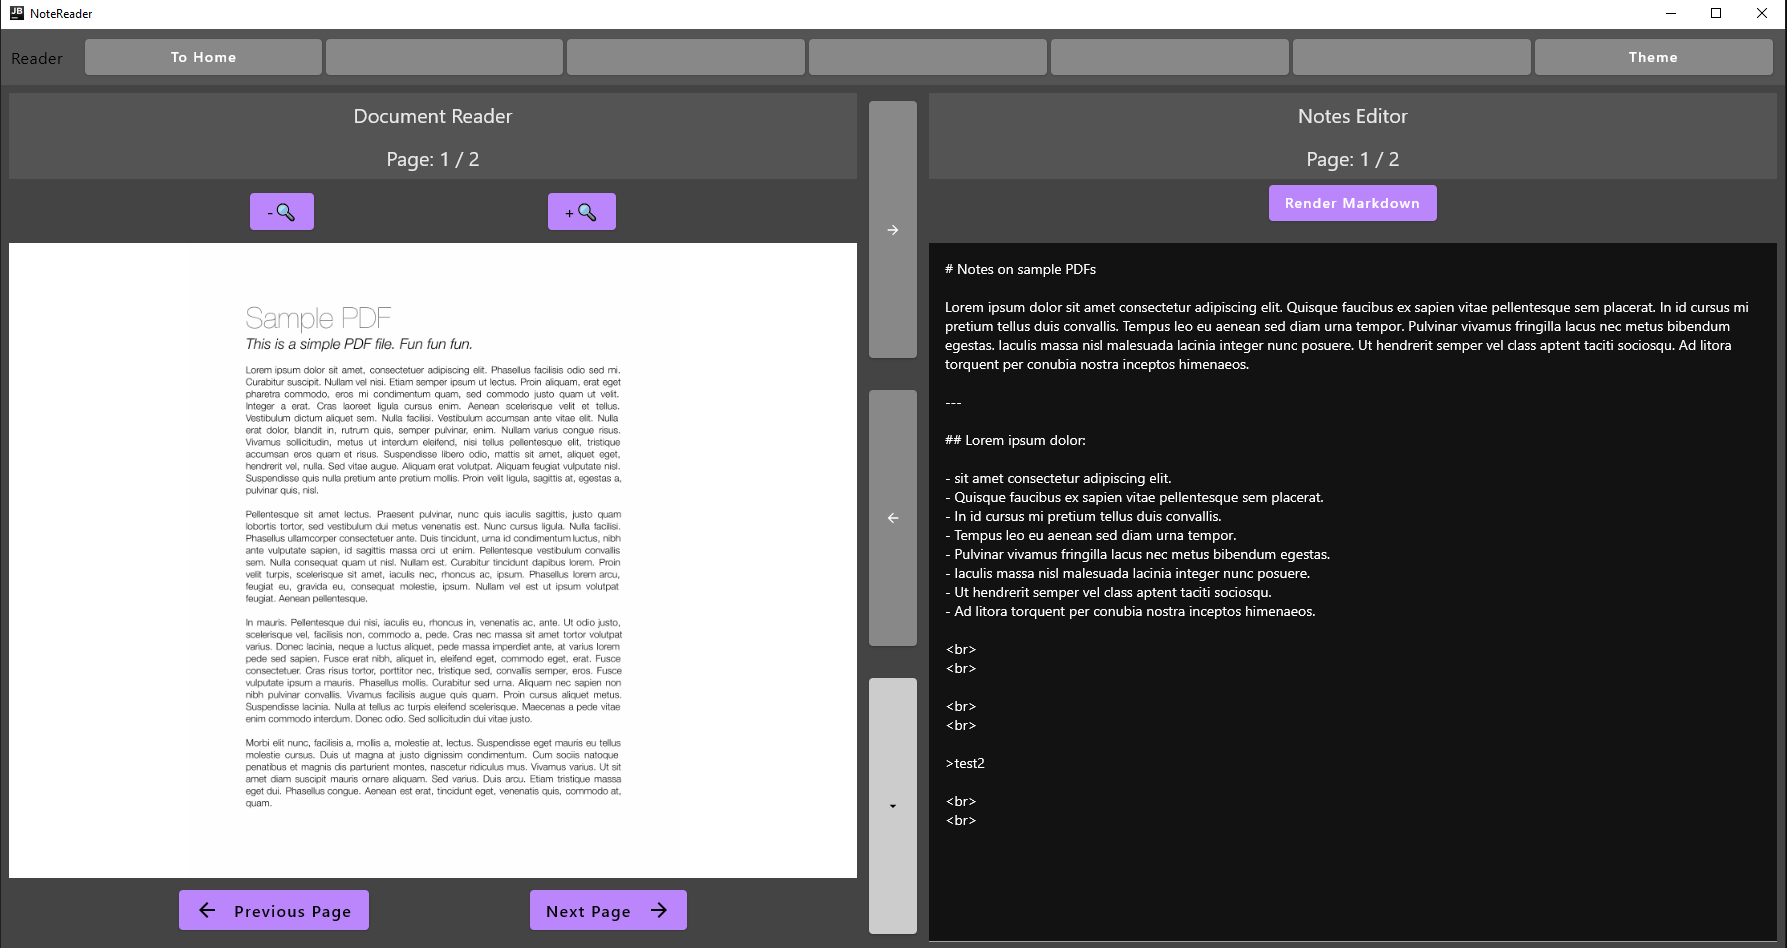
\includegraphics[width=1\linewidth]{Figures/image4.png}
    \caption{Dark Mode}
    \label{fig:dark}
\end{figure}

\subsubsection{Evolution of the Design and Lessons Learned}

The design of NoteReader evolved significantly over the course of development, shaped by technical constraints, time limitations, and practical insights gained through implementation. The foundation of the project however, split-view note taking, document integration, and plain-text note portability remained constant.

One of the most prominent evolutions was the architectural strategy for handling document rendering. The original goal was to have have native support for each format. This approach was determined to be impractical for a prototype. Instead, a fallback architecture was introduced: all supported document types were converted to PDF at runtime and rendered using a unified PDF renderer. This preserves the project's core requirement of true-to-intent document rendering, while simplifying implementation.

The scope of the project also shifted to emphasize core functionality. While the initial vision included synchronization, tagging and searching, and full multiplatform support, these features were pushed back to a later development cycle in order to focus on delivering a robust and usable Minimum Viable Product. Emphasis was placed on ensuring the design was fully modular, with string architecture to ensure these features could be integrated in future iterations. 

One of the most important lessons learned was the importance of adaptability in software projects. Various difficulties including framework maturity, integration complexity, and time management all influenced the project's direction. Attempting to strictly follow the original implementation plan would have made it difficult to deliver a completed product. The deferral of some requirements allowed the primary vision of the application to be maintained in the first iteration of the product, while preparing to implement those requirements in future. 


% In December of last year, when writing the first version of the report, in Chapter 4 you came up with your original solution approach. On it, you presented (i) the architecture of your solution, (ii) your list of use cases, (iii) a risk assessment, (iv) a methodology to develop your solution approach, (v) your implementation schedule, (vi) your evaluation plan and (vii) some prototype of the resulting product. From January to April you have been developing your solution approach. Along the way you have encountered difficulties (the ones listed in Section 5.1) which might have modified your original plan so that you can come up with an actual developed project.

% This section is effectively the production of "as built" specification where you compare your original design to the final finished project. Please go section by section (the ones listed from (i) to (vii) in the last paragraph. For each section, enumerate any difference between the original design and the final project, and justify the difficulty forcing you to make such this change. Do not fret if some of these changes are radical, what is important here is that there is a clear rationale for changes made.

